\chapter{Aprendizaje automático}

En este capítulo se profundizará en el área de \emph{aprendizaje automático}
abarcando la representación de palabras y oraciones dadas por codificaciones del
tipo one-hot, word embeddings, conceptos de aprendizaje supervisado y no
supervisado, modelos de clasificación, ajuste de hiperparámetros, y métricas.

\section{Orígenes y evolución}

El aprendizaje automático es el campo de la inteligencia artificial que busca
desarrollar programas que mejoren en base a la experiencia. Estos métodos
difieren del típico paradigma de implementación donde en lugar de ser
``programado`` es ``entrenado``. Tal entrenamiento consiste en disponerle al
algoritmo información en forma de ejemplos con el fin de reconocer patrones
estadísticios y eventualmente determinar reglas que sirvan para automatizar una
tarea.

Por moderno que pueda parecer este campo, tuvo sus comienzos en los años 50 a
partir del famoso \emph{Test de Turing}, una máquina cuyo objetivo era engañar a
un humano haciéndole creer que se encontraba delante de otra persona en lugar de
un ordenador, se llegó  a la conclusión de que los computadores de propósito
general, podrían ser capaces de aprender y ser de alguna manera originales.
\footnote{\url{https://www.turing.org.uk/scrapbook/test.html}}

En los últimos años varias aplicaciones se han beneficiado de esta área, desde
programas relacionados con la detección fraudulenta de transacciones con tarjeta
de credito, sistemas de recomendación que guían usuarios en un servicio de
acuerdo a sus preferencias, o incluso vehículos que se manejan sin necesidad de
la intervención del conductor. Al mismo tiempo, una importante cantidad de
avances teóricos y algorítmicos se fueron realizando formando las bases de este
campo. TODO: Poner referencias a los ejemplos.

Aún con estos increibles logros, no se conoce aún como crear computadoras que
aprendan al nivel que las personas lo hacen. No obstante, se han desarrollado
algoritmos que se han aproximado a este objetivo siendo efectivos para varios
tipos de problemas.

\section{Aprendizaje supervisado}

El aprendizaje supervisado es una subárea del aprendizaje automático cuyo
objetivo es deducir un modelo a partir de datos anotados que permita mapear
ejemplos no vistos previamente. Esta información está compuesta por un conjunto
de ejemplares y sus correspondientes etiquetas, en ocasiones dada por un
anotador humano, la cual indica el resultado del modelo a partir del dato como
entrada. Las etiquetas pueden ser categóricas o continuas determinando un
problema de clasificación o regresión. Algunas tareas más frecuentes de
clasificación son la categorización de documentos, reconocimiento de lenguaje
ofensivo, o análisis de sentimiento. Mientras que para regresión, lo son las
estimaciones de precios de artículos, objetos, o viviendas.

El resultado de ejecutar un algoritmo de machine learning supervisado se puede
expresar como una función $f(\vect{x})$ que recibe un ejemplar $\vect{x}$ como
entrada y genera un vector $\vect{y}$ de salida codificado de la misma manera
que las etiquetas. Las muestras utilizadas para ajustar $f$ estan dadas por
vectores $\{\vect{x}_1, ..., \vect{x}_n\}$ y anotaciones $\{y_1, .. y_n\}$
conformando el \emph{conjunto de entrenamiento}.

La forma precisa de $f$ es determinada durante la fase de entrenamiento. Una vez
transcurrida, se puede estimar la identidad de nuevos datos etiquetados
pertenecientes al \emph{conjunto de test} con el fin de evaluar la performance
del modelo. En el caso que la predicción se aproxime a la esperada para estas
nuevas entradas, entonces el modelo habría logrado generalizar la tarea.

Sin embargo, los modelos de aprendizaje supervisado están limitados por la
disponibilidad de las anotaciones y la dificultad para obtenerlas.
Algunas tareas son relativamente sencillas de etiquetar por cualquier
persona, (e.g. como determinar si en una foto aparece un gato), mientras que en
otros puede llegar a requerir humanos que sean expertos de dominio (e.g.
abogados, médicos, lingüistas, etc).

\section{Aprendizaje no supervisado}

En contraste al método anterior, el aprendizaje no supervisado consiste en
descubrir automáticamente patrones sobre los datos de entrenamiento que permitan
explicarlos sin depender de datos de anotados. Es considerada como una parte del
área del análisis y exploración. Es por eso que no pueden ser evaluados
basándose en exactitud o precisión, si no más bien en la cantidad de información
que podamos extraer de los datos a partir del uso de estas técnicas. Algo a
considerar es la facilidad para disponer de estos datos (en comparación a los no
supervisados) al no requerir ningún tipo de supervición humana.

\section{Codificación de características}

Los modelos de aprendizaje automático dependen fuertemente de como se
representen los datos de entrada que uno tiene disponible. Preparar los
ejemplares para acoplarse apropiadamente a un algoritmo de machine learning con
el fin de mejorar la performance del modelo es una de las tareas las cuales los
científicos de datos disponen la mayor parte de su atención y tiempo. Alguna de
las obligaciones que incluye son la imputación de valores faltantes, manejo de
valores atípicos, estandarización y escalado, transformación de características
numéricas a categóricas, y codificación.

En particular pondremos nuestro foco en la codificación de características
desarrollando métodos del tipo \emph{one-hot} y \emph{word embeddings}.

\subsection{One-hot encoding}

A menudo los datos disponibles presentan características que no estan dadas en
un espacio continuo si no más bien categórico. Por ejemplo, se podría describir
el continente de un país por las clases \emph{inAsia}, \emph{inAfrica},
\emph{inEurope}, \emph{inSouthAmerica}, \emph{inNorthAmerica} siendo
eficientemente representables con enteros $[0, 1, 2, 3, 4]$. De esta manera, si
tenemos una serie de variables categóricas, estas pueden codificarse enumerando
por variable cada uno de sus objetos. Esta representación es conocida como
\emph{ordinal encoder}.

\begin{equation*}
    \begin{bmatrix}
         & inContinent\\
        Argentina & 3 \\
        Brasil & 3 \\
        España & 2 \\
        USA & 4  \\
        Italia & 2 
    \end{bmatrix}
\end{equation*}

Otra opción es usar un esquema \emph{one-of-K} que
transforma una característica categórica con $N$ clases, en $N$ categorias
binarias con una de ellas 1 y el resto 0. Para el ejemplo anterior tendríamos:

\begin{equation*}
\begin{bmatrix}
    & inAsia & inAfrica & inEurope & inSouthAmerica & inNorthAmerica \\
    Argentina & 0 & 0 & 0 & 1 & 0 \\
    Brasil & 0 & 1 & 0 & 1 & 0 \\
    España & 0 & 0 & 1 & 0 & 0 \\
    USA & 0 & 0 & 0 & 0 & 1 \\
    Italia & 0 & 0 & 1 & 0 & 0
\end{bmatrix}
\end{equation*}

La misma técnica es válida si se quisiera representar oraciones o documentos del
lenguaje natural. Supongamos que tenemos los documentos.

\begin{center}
    $D_1$: ``El sol es una estrella, no es un planeta.`` \\
    $D_2$: ``La tierra es un planeta.``    
\end{center}

Basado en  estos dos textos, un vocabulario de 9 palabras distintas es
construido. Por lo tanto cada documento es representado como un vector de 9
dimensiones.

\begin{equation*}
    \begin{bmatrix}
        & El & sol & es & una & estrella & no & un & planeta & tierra \\
        D_1 & 1 & 1 & 2 & 1 & 1 & 1 & 1 & 1 & 0  \\
        D_2 & 0 & 0 & 1 & 0 & 0 & 0 & 1 & 1 & 1 
    \end{bmatrix}
\end{equation*}

Observar que para este caso una codificación ordinal no sería adecuada dado que
se deberían enumerar todas las palabras del vocabulario.

Sin embargo, tomemos una oración dada en el contexto de planning (en particular
del dominio \emph{satellite} descripto en apéndice A). La siguiente secuencia
muestra un plan relajado de largo 4 asociado a una tarea STRIPS cuyos esquemas
de acción son $calibrate, switch\_on, take\_image,$ y $turn\_to$. El resto de
expresiones son objetos concretos del dominio. También es importante mencionar
que cada objeto de un cierto tipo está enumerado. Por ejemplo el objeto
$instrument1$ es del tipo $instrument$ cuyo índice es $1$. 

\begin{align*}
    & (calibrate\ satellite0\ instrument1\ groundstation0) \\
    & (switch\_on\ instrument1\ satellite0) \\
    & (take\_image\ satellite0\ planet5\ instrument1\ image1) \\
    & (turn\_to\ satellite0\ groundstation0\ planet5) \\
\end{align*}

La primera dificultad para codificarla surge bajo la pregunta de a que se
identifica como una palabra de la oración. Una primera iniciativa es definir una
acción como tal y utilizar un one hot encoding. No obstante, por lo general
una acción no suele ocurrir más de una vez en un plan de la tarea lo cual se
perdería la información de la frecuencia en que ocurren los objetos en la
secuencia. No solo es clave capturar los objetos si no también el índice del
cual se trata. Por lo tanto respetar su numeración es igual de relevante. Por
último cada acción debe mantener la misma cantidad de componentes en su
representación vectorial, independientemente del esquema o el número de
parámetros que reciba, y se debe asegurar el orden de la secuencia.

Para solventar estas dificultades se mantuvo una codificación one hot ordinal que
consiste en:

\begin{itemize}
    \item Cada elemento en la interfaz de una acción junto a su esquema son
    definidos como palabras. Eso incluye la numeración de los objetos.
    \item Cada vector que representa a una acción tiene dimensión $2 \times N +
    1$ siendo $N$ la longitud de la interfaz más larga de un esquema. Aquellas
    acciones con una interfaz más chica se les agrega un margen de $0's$ hasta
    completar el largo requerido.
    \item Los esquemas de acción son enumerados en el rango $1, ..., M$ con $M$
    la cantidad de esquemas.
    \item El tipo de los objetos son enumerados en el rango de $1, ..., K$. con
    $K$ la cantidad de tipos.
    \item Si un objeto tiene el índice $i$ se lo incrementa en 1 (para evitar que
    aquellos objetos que empiecen con indice 0 se malinterpreten como margenes).
\end{itemize}

Por ejemplo si la enumeración de las esquemas y tipos fuesen los siguientes:

\begin{align*}
    &\{calibrate: 1,\ turn\_to: 2,\ switch\_on:3,\ take\_image:4 \} \\
    &\{satellite: 1,\ instrument: 2,\ planet: 3,\ groundstation: 4,\ image: 5\}
\end{align*}

En este la longitud de la interfaz más larga es 4, entonces cada acción tendrá
asociado un vector de dimensión $2 \times 4 + 1 = 9$ y la codificación
resultante sería:

\begin{align*}
    (calibrate\ satellite0\ instrument1\ groundstation0) &: (1\ 1\ 1\ 2\ 2\ 4\ 1\ 0\ 0) \\
    (switch\_on\ instrument1\ satellite0) &: (3\ 2\ 2\ 1\ 1\ 0\ 0\ 0\ 0) \\
    (take\_image\ satellite0\ planet5\ instrument1\ image1) &: (4\ 1\ 1\ 3\ 6\ 2\ 2\ 5\ 2) \\
    (turn\_to\ satellite0\ groundstation0\ planet5) &: (2\ 1\ 1\ 4\ 1\ 3\ 6\ 0\ 0) \\
\end{align*}

\subsection{Vectores de palabras (Word embeddings)}

Un vector denso de palabras (comúnmente conocido como word embedding, en inglés)
es una de las técnicas de representación de vocabulario más popular en el área
del procesamiento de lenguaje natural.

Si bien hay distintas formas de representar palabras en una serie de documentos,
los word embeddings proveen otra perspectiva que busca encontrar una
representación vectorial compacta donde cada dimensión logre capturar las
propiedades subyacentes y latentes de la palabra. De esta manera, los embeddings
son superiores a una representación que permanece en un nivel poco profundo.

Su principal característica  es que las expresiones relacionadas entre sı́ (ya
sea por contexto, semántica o sintaxis) se encuentren cercanas en el espacio
vectorial al cual se proyectan. Por ejemplo, si tenemos las oraciones: ``Que
tengas una buena mañana`` y ``Que tengas una buena tarde``. Difieren
semánticamente solo por las palabras ``mañana`` y ``tarde``. No obstante, se
utilizan en contextos similares, lo cual esperariamos que esten cercanos
vectorialmente.

Otro ejemplo muy famoso que deja en evidencia el concepto de \emph{analogía} en
word embeddings, es el que se muestra en la Figura \ref{fig:king-queen-example}.
En ella se identifican por medio de barras de colores la dimensión de los
vectores asociados a las palabras \emph{king}, \emph{man}, \emph{woman},
\emph{queen}, y la operación vectorial \emph{king - man + woman}. Cada dimensión
se encuentra en la escala de $[-2, 2]$ y se le asigna el color de rojo para
valores cercanos al extremo derecho, azúl para las del extremo izquierdo, y
blanco para las que se encuentren alrededor del 0.  Algo a notar es que
\emph{man} y \emph{woman} son mucho más similares de lo que cada uno es con
\emph{king} o \emph{queen}. Otro aspecto interesante son las franjas roja y azúl
que se muestran para cada uno de los ejemplos, indicando que son parecidos en
tal dimensión. Probablemente corresponda a alguna característica humana aunque
se desconoce que puedan llegar a significar debido a la poca interpretabilidad
del espacio al cual se proyectan.

Aun así, lo importante es la comparación entre palabras. Dado que ahora tienen
una representación vectorial, se pueden sumar o restar obteniendo nuevos
resultados que forman parte del espacio. Este es el caso del vector dado por
\emph{king - man + woman}. No conocemos que dimensiones exactamente capturan que
rey es utilizado para identificar al monarca de un reino, pero se puede
substraer el caracter masculino del vector \emph{man} y agregar las de
\emph{woman} esperando que se aproximen a las de \emph{queen}.
Sorprendentemente, de un total de 400000 palabras sobre las cuales se realizó el
experimento, reina fue la palabra más cercana. Los detalles del mismo se pueden
ver desde \footnote{\url{https://jalammar.github.io/illustrated-word2vec/}}.

\begin{figure}
    \centering
    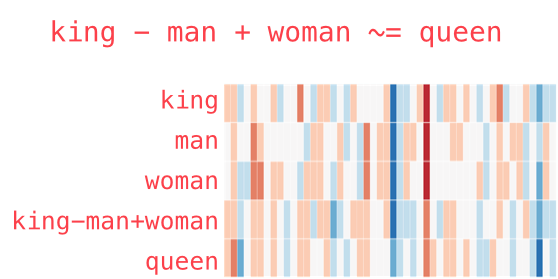
\includegraphics[scale=0.68]{figures/king-analogy-viz.png}
    \caption{Vectores de palabras para ``king``, ``man``, y ``woman``}
    \label{fig:king-queen-example}
\end{figure}

Esto refleja el gran potencial que tienen los word embeddings y su importancia
para estudiarlos como métodos de codificación. A continuación analizaremos como
se calculan dichas representaciones y que algoritmos fueron finalmente
utilizados en esta tesis.

\subsubsection{Modelos de lenguaje}

Después de ver el potencial de los embeddings, surge la pregunta, ¿Cómo
funcionan internamente? ¿De qué manera se obtienen estos vectores de palabras?
En \citep{firth-57} se mostró que el significado de una palabra está determinado
según sus palabras vecinas. Si contemplamos la oración ``Que tengas un buen`` y
se quisiese averiguar cual es la expresión que le sigue, lo más probable es que
las palabras días, tarde, noche, o semana, hayan sido las primeras candidatas.
Este tipo de tareas en las que se intenta predecir información de la oración a
partir del contexto o viceversa son denominadas tareas de pretexto y son
utilizadas para entrenar un clasificador que resuelva esta tarea, únicamente
para preservar su representación a nivel de palabras.

\subsubsection{Skipgram}

Es un método desarrollado en \citep{Mikolov-2013} cuyo objetivo es, para un
vocabulario de tamaño $W$ donde una palabra es identificada por su indice $w \in
\{1, ... W\}$, aprender una representación vectorial para cada $w$. Estas
representaciones son entrenadas para predecir palabras vecinas a partir de una
actual. Es decir, dado un largo corpus de entrenamiento, considerarlo como una
sola secuencia de palabras $w_1, ... w_T$ y maximizar la función en \ref{eq:skipgram-ideal}

\begin{equation} \label{eq:skipgram-ideal}
    \frac{1}{T} \sum_{n=1}^{T}
                    \sum_{c \in C_t} \log P(w_c | w_t)
\end{equation}

Donde $C_t$ es el conjunto de indices de palabras que rodean a $w_t$. La
probabilidad de observar una palabra del contexto $w_c$ dado $w_t$ es modelada a
partir de sus vectores representación. Por el momento, abstraeremos esto a
partir de una función \emph{score} $s$ que mapea pares (palabra, contexto) a un
puntaje en $R$. Una posible forma de definir la probabilidad de una palabra en
el contexto es por medio de la función \emph{softmax}.

\begin{equation} \label{eq:skipram-softmax}
    P(w_{c}|w_{t}) = \frac{e^{s(w_t, w_c)}}{\sum_{j=1}^{W} e^{s(w_t, j)}}
\end{equation}

No obstante, este calculo es bastante costoso computacionalmente siendo que al
final solo es de interés predecir una palabra del contexto $w_c$ dado una
palabra $w_t$. Es por eso que el problema puede ser visto como una tarea de
clasificación binaria en lugar de una multiclase. El objetivo es predecir
independientemente la presencia o ausencia de palabras de contexto. Para una
palabra en la posición $t$, consideramos todos los contextos como ejemplos
positivos, y palabras seleccionadas aleatoriamente del vocabulario, como
negativos. Para un contexto $c$, utilizando la función de costo \emph{binary
logistic}, obteniendo la siguiente función de probabilidad:

\begin{equation}
    \log\left( 1 + e^{-s(w_t, w_c)} \right) +
    \sum_{n \in \mathcal{N}_{t, c}} \log\left( 1 + e^{s(w_t, n)} \right)
\end{equation}

Donde $\mathcal{N}_{t, c}$ es una muestra aleatoria de ejemplares negativos
tomadas del vocabulario. Si denotamos la función logistica como $\ell: x \mapsto
\log \left(1 + e^{-x} \right)$, podemos reescribir la función a maximizar del
problema como:

\begin{equation}
    \sum_{n=1}^{T} 
        \sum_{c \in C_t} \ell\left(s(w_t, w_c)\right) +
        \sum_{n \in \mathcal{N}_{t, c}} \ell\left(-s(w_t, n) \right)
\end{equation}

Una parametrización natural para $s$ entre una palabra $w_t$ y un contexto $w_c$
es a partir del uso de vectores de palabras. Definimos dos vectores $\vect{u}_w$
y $\vect{v}_w$ en $\mathbb{R}^d$ también conocidos como vectores \emph{input} y
\emph{output}. Es decir, tenemos vectores $\vect{u}_{w_t}$ y $\vect{v}_{w_c}$
asociados a palabras $w_t$ y $w_c$. Luego el \emph{score} puede computarse como
$s\left( w_t, w_c \right) = \vect{u}_{w_t}^\top \vect{v}_{w_c}$.

Para ejemplificar como es el proceso de entrenamiento de este modelo, tomemos la
secuencia ``Me gustaría dos rebanadas de pizza mozzarella``. Podemos pensar un
contexto como una ventana que se desliza a través del conjunto de entrenamiento.
La figura 3.2 muestra las 3 posibles ventanas de tamaño 5 que se pueden obtener
a partir de la secuencia deslizandose con un paso de 1.

Con cada ventana, seleccionamos aquella palabra que cargue más valor
informativo, que por lo general suele ser la del medio, y la utilizamos para
predecir sus vecinas. De esta manera, generamos un conjunto de entrenamiento
compuesto por pares (palabra, palabra de contexto) donde etiquetamos con 1, si
ambas son vecinas, y 0 en caso contrario. El resultado final para cada contexto
se puede ver en la figura 3.3. Esta es la simplificación del problema para
trabajar sobre una tarea de clasificación binaria. En lugar de ser multiclase
cuya  etiqueta sería la palabra de contexto, la incluimos como característica y
reemplazamos las anotaciones por 1's y 0's. Ahora bien, con nuestros datos
actuales solo tendríamos etiquetas con 1's. En tal caso, el modelo en lugar de
aprender lo que necesitamos, estaría sesgado a siempre predecir afirmativamente.
Es por eso que agregar ejemplos negativos de manera aleatoria (figura 3.4) a
cada $w_t$ resulta una buena idea.

\begin{figure}
    \centering
    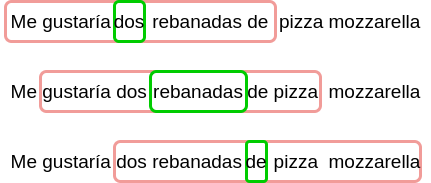
\includegraphics[scale=0.60]{figures/context_example_1.png}
    \caption{Todas las ventanas de contexto con tamaño 5 que se pueden formar con la frase
             ``Me gustaría dos rebanadas de pizza mozzarella``.}
\end{figure}

\begin{figure}
    \centering
    \begin{minipage}[b]{0.4\textwidth}
      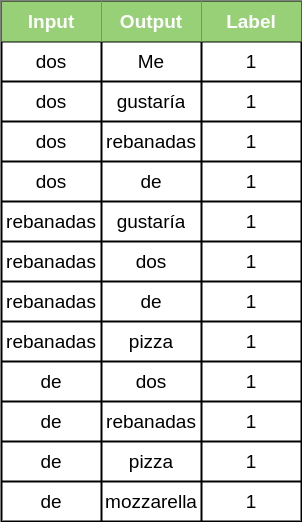
\includegraphics[scale=0.5]{figures/context_example_2.png}
      \caption{Material de entrenamiento obtenido de las ventanas.}
    \end{minipage}
    \hfill
    \begin{minipage}[b]{0.4\textwidth}
      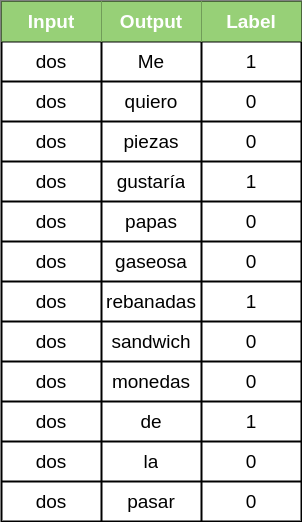
\includegraphics[scale=0.5]{figures/context_example_3.png}
      \caption{Selección aleatoria de 2 ejemplos negativos por cada positivo.}
    \end{minipage}
\end{figure}

Luego, al inicio del proceso de entrenamiento se crean dos matrices con valores
aleatorios, una para los embeddings y otra para los contextos. Estas dos
matrices de tamaño $V \times d$, tiene una fila por cada palabra en el
vocabulario. En este caso, $d$ es la cantidad de dimensiones que tendrán sus
representaciones. En cada paso de entrenamiento, se selecciona un ejemplo
positivo y sus correspondientes ejemplos negativos (figura 3.5). Este grupo es
evaluado por el modelo a partir de los vectores representación \emph{input} y
\emph{output} según el producto escalar entre ellas y su conversión en
probabilidades por medio de la función \emph{sigmoid}. A partir de la etiqueta
real, se puede determinar el puntaje de error para cada ejemplo y finalmente
actualizar los parámetros de las matrices de embeddings y contexto. Eso concluye
un paso de entrenamiento, que se repite por cada grupo de ejemplos positivos y
negativos por una cierta cantidad de épocas. Una vez concluido el proceso de
entrenamiento, la matriz de embeddings contiene las representaciones finales.

\begin{figure}
    \centering
    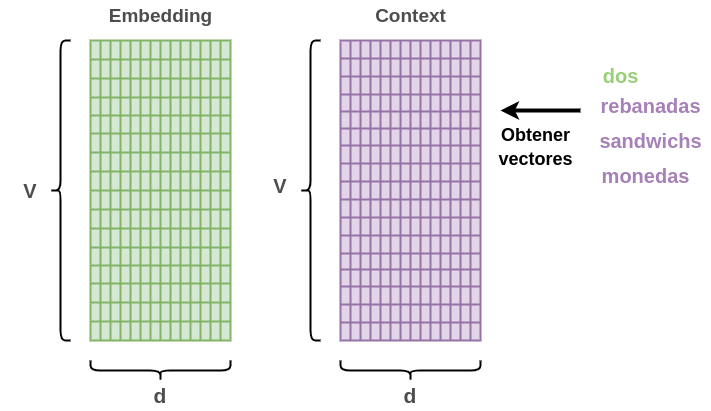
\includegraphics[scale=0.5]{figures/context_example_4.png}
    \caption{Matrices para los embeddings y contextos.}
\end{figure}

\subsubsection{Modelos de lenguaje a nivel de subpalabra}

El modelo de skipgrams al usar vectores representación por cada palabra se
ignora su estructura interna. Esto fue lo que inspiró el estudio de modelos a
nivel de subpalabra en \citep{bojanowski-2017}. La principal característica de estos modelos
radica en la función de score $s$. En lugar de considerar una palabra $w$ en su
totalidad, esta es dividida en $n$-gramas de caracteres. Para delimitar inicio y
fin de una palabra se agregan símbolos especiales \verb|<| y \verb|>| respectivamente. Esto a
su vez permite distinguir prefijos y sufijos de otras secuencias de caracteres.
Por último la palabra $w$ también es incluida como un $n$-grama o secuencia
especial. Por ejemplo, la palabra \emph{color} y $n=4$ estaría representada por
los $4$-gramas:

\begin{center}
    \verb|<col|, \verb|colo|, \verb|olor|, \verb|lor>|
\end{center}

Junto a la secuencia completa \verb|<color>|. Notar que la secuencia
\verb|<olor>| correspondiente a la palabra \emph{olor} es diferente al $4$-grama
\verb|olor|. Luego lo único que queda restante es modificar la función
\emph{score} $s$ del método skipgram por la siguiente:

\begin{equation}
    s\left(w, c\right) = \sum_{g \in \mathcal{G}_w} \vect{z}_g^{\top}\vect{v}_c
\end{equation}

Donde $\mathcal{G}_w \subset \{1, .. G\}$ siendo $G$ el conjunto de $n$-gramas
de tamaño $G$ y $\vect{z}_g$ el vector representación del $n$-grama $g$.

Este modelo permite compartir representaciones entre palabras logrando aprender
una confiable representación a palabras poco comunes siendo útil para los
experimentos de esta tesis en la tarea de codificación de planes relajados.

\subsubsection{Representación vectorial de oraciones}

En \citep{Iacobacci-2016} se explican como utilizar word embeddings para
desambiguación de sentidos, proponiendo distintos métodos de codificación de
instancias de entrenamiento a partir de un modelo de lenguaje, con el fin
de incluirlos en una arquitectura supervisada. En particular, detallaremos
algunos métodos más sencillos y que son común en la literatura para resolver
tareas de clasificación que involucren la manipulación de texto.

\textbf{Concatenación}. Este método consiste en concatenar los vectores de las
palabras que conforman la oración a codificar obteniendo un vector de largo
igual a la suma de las dimensiones de los vectores individuales. En este caso,
el problema evidente que surge es la representación de oraciones con distinto
largo y el tamaño del vector resultante.

\textbf{Promedio}. Como su nombre lo indica, este método computa el centroide de
los embeddings de todas las palabras que conforman una oración. Usualmente esta
codificación resulta ser adecuada siempre y cuando los vectores de las palabras
se encuentren en la misma escala, lo cual no siempre suele ser el caso. Otro
problema menos evidente es la posibilidad de ocurrencia de palabras poco
representativas pero que tengan mucho peso en la suma, ignorando las ocurrencias
que nos interesan para la tarea que se intenta resolver.

\textbf{Promedio normalizado}. Por último, una mejora de la representación
anterior es la normalización por norma L2 de cada vector previo a realizar el
promedio.

\section{Algoritmos de clasificación}

El objetivo principal de un clasificador es aproximar una función no conocida
$f$ a partir de un modelo $h: \mathbb{R}^d \rightarrow \{c_1,.., c_k\}$ la cual
mapea ejemplos de entrada a una categoría $c_j$. En particular, nos enfocaremos
en clasificadores binarios $k = 2$ que fueron los utilizados para la realización
de este trabajo.

\subsection{Modelos lineales}

La forma más sencilla de representar un función que discrimine datos de entrada
en dos clases es a partir de una función lineal que dependa de estos datos:

\begin{align}
    h_{\vect{w}, w_0}\left( \vect{x} \right) &= \vect{w}^{\top} \vect{x} + w_0 \\
                                           &= \sum_{j = 1 }^{d} w_j x_j + w_0
\end{align}

Donde $\vect{w}$ es llamado el \emph{vector de pesos}, y $\vect{w_0}$ es el
\emph{sesgo}. Ambos son parámetros de la función $h$ y son los que se buscan
ajustar para lograr separar el conjunto de datos. $\vect{x}$ es uno de esos
ejemplos. Las dimensiones de los vectores $\vect{x}$, y $\vect{w}$ son ambas $(d
\times 1)$ a diferencia del sesgo que es un escalar. La expresión
$\vect{w}^{\top} \vect{x}$ es el producto interno entre $\vect{w}$ y $\vect{x}$.
Por lo que el resultado de $\vect{w}^{\top} \vect{x} + b$ es también un escalar.
Dado que nos interesa asignar a $\vect{x}$ una categoría, se debe decidir a cual
pertenece en base al resultado obtenido por el producto interno. Es por eso que
surge la necesidad de agregar una nueva operación que discrimine un valor de
entrada en una clase. Para ello definimos la función $f: \mathbb{R} \rightarrow
\{c_1, c_2\}$ conocida como \emph{función de decisión} tal que mapea valores a
una clase $c_1$, o $c_2$.

Una posible función de decisión podría estar definida como $f(x) = c_1$ si $x
\geq 0$, $f(x) = c_2$ caso contrario. Por lo tanto la frontera de decisión queda
definida por la relación $h_{\vect{w}, w_0}\left( \vect{x} \right) = 0$ y
corresponde a un hiperplano de ($d-1$ dimensiones) en uno de $d$ dimensiones. El
sesgo $w_0$ desplaza el hiperplano del origen coordenados de $d$.

Algunas veces es conveniente usar una notación más compacta en la que
introducimos una ``inocente`` componente de entrada más $x_0 = 1$ al vector
$\vect{x}$ para luego definir $\vect{w}' = (w_0, \vect{w})$ y $\vect{x}' = (x_0,
\vect{x})$ de tal manera que 

\begin{align}
    h_{\vect{w'}}\left( \vect{x'} \right) &= \vect{w'}^{\top} \vect{x'}\\
                                           &= \sum_{j = 0 }^{d} w_j x_j
\end{align}

Ahora la frontera de decisión corresponde a un hiperplano de dimensión $d$ que
pasa por el origen del espacio $d + 1$ dimensional. A partir de ahora, cada vez
que se omita el sesgo estaremos utilizando esta notación.

\subsection{Modelos probabilisticos}

En el capítulo 2 mencionamos que el objetivo de usar un algoritmo de aprendizaje
automático era con el fin de determinar una función que modele la probabilidad
de que una acción sea relevante para encontrar un plan de una tarea STRIPS. Sin
embargo desconocemos aún de que manera se obtienen estas probabilidades, es por
eso que el foco de esta sección es indagar sobre los modelos probabilisticos.

El objetivo es modelar la densidad condicional $p(c_k | \vect{x})$ que
representa la probilidad de la clase $c_k$ dado $\vect{x}$. El inconveniente con
esto es que cada condicionamiento define una densidad probabilistica. Por lo que
se tendría una por cada posible ejemplar $\vect{x}$ resultando intratable de
modelar. No obstante, si se considera el condicionamiento $p(\vect{x} | c_k)$
solo es necesario modelar una cantidad pequeña de clases, en especial para un
clasificador binario. Para nuestra suerte $p(c_k | \vect{x})$ está relacionado
con $p(\vect{x} | c_k)$ por la \emph{regla de Bayes}.

\begin{align}
    p\left( c_1 | \vect{x} \right) &= \frac{p\left( \vect{x} | c_1 \right)p(c_1)}{
                                            p\left( \vect{x} | c_1 \right) p(c_1) + 
                                            p\left( \vect{x} | c_2 \right)p(c_2)} \\
                                   &= \frac{1}{1 + \exp\left( -a \right)} \\
                                   &= \sigma(a)
\end{align}

Donde definimos $a = \ln \frac{p\left( \vect{x} | c_1 \right) p\left( c_1
\right)}{p\left( \vect{x} | c_2 \right) p\left( c_2 \right)}$. La función
$\sigma(a)$ es conocida como la función \emph{sigmoide} y juega un importante
rol en muchos algoritmos de clasificación por su propiedad de simetría
$\sigma(-a) = 1 - \sigma(a)$, el significado de su inversa $a = \ln \left(
\frac{\sigma}{1 - \sigma} \right)$ que representa el logaritmo del radio de las
probabilidades de las clases $c_1$ y $c_2$, y la capacidad de mapear el eje real
en un intervalo finito.

Se puede generalizar esta ecuación para el caso $k > 2$ de la siguiente manera:

\begin{align}
    p\left( c_k | \vect{x} \right) &= \frac{p\left( \vect{x} | c_k \right)p(c_k)}{
                                                \sum_{j=1}^{k} p\left( \vect{x} |
                                                c_j \right) p(c_j) } \\
                                       &= \frac{\exp\left( a_k \right)}{\sum_{j=1}^{k} a_j} \\
\end{align}

Donde $a_k = \ln p\left( \vect{x} | c_k \right) p\left( c_k \right)$. La función
$\frac{\exp\left( a_k \right)}{\sum_{j=1}^{k} a_j}$ es conocida como la función
\emph{softmax} ya que es una versión suavizada del \emph{max} en el sentido de
si $a_k >> a_j$ para todo $j \neq k$ entonces $p(c_k | \vect{x}) \approx 1$ y
$p(c_j | \vect{x} \approx 0)$.

\subsection{Función de costo}

Varios de los métodos de machine learning existentes no pueden obtener los pesos
$W$ de manera analítica. Es por eso que se hacen uso de métodos iterativos en
base a una \emph{función de costo} que mide la precisión de su predicción en
comparación con la etiqueta. Si tenemos ejemplos de entrenamiento
$\{(\vect{x}^{(1)}, y^{(1)}), ..., (\vect{x}^{(n)}, y^{(n)})\}$ podemos definir la
función de costo en base a cada ejemplar $i$.

Un ejemplo clásico de función de costo es el error cuadratico medio:

\begin{align}
    J(\vect{w}) = \frac{1}{2n} \sum_{i=1}^{n}\left( h_{\vect{w}}\left( \vect{x}^{(i)}\right) - y \right)
\end{align}

Por lo tanto al minizar $J$ se estará reduciendo el error de estimación de $h$
obteniendo que $h_{\vect{w}}\left( \vect{x}^{(i)} \right) \approx f(\vect{x}^{(i)})$. Para
lograr tal minimización, existe una técnica denominada \emph{descenso por el
gradiente}. la cual actualiza de manera iterativa de los parámetros W, logrando
la convergencia de la función de costo J a un mínimo valor.

\subsection{Descenso por el gradiente}

Definimos $\vect{\Delta J\left( w \right)}$ al gradiente de $J$ en $\vect{w}$
como $\vect{\Delta J\left( \vect{w} \right)} = \left(\frac{\partial
J(\vect{w})}{\partial w_1}, ..., \frac{\partial J(\vect{w})}{\partial w_n}
\right)$, el vector de derivadas parciales. Este algoritmo empieza con una
inicialización aleatoria de $\vect{w}$ donde en cada iteración se determina
$\vect{\Delta J\left( w \right)}$. El negativo del gradiente indica la dirección
de mayor descenso en el cual la función $J(\vect{w})$ disminuye. Por lo tanto si
al vector $\vect{w}$ se le suma el negativo del gradiente se estaría
dirigiendolo en torno a un mínimo local de la función de costo. La magnitud del
desplazamiento vectorial en cada iteración está determinado por una constante
$\alpha$ conocida como la \emph{taza de aprendizaje}.

\begin{align}
    \vect{w} \leftarrow \vect{w} - \alpha \vect{\Delta J\left( w \right)}
\end{align}

En cada iteración se realiza la operación de la ecuación actualizando
$\vect{w}$. Algo a notar es que es una operación vectorial de tal manera que
cada componente se actualice simultaneamente. Intuitivamente, en cada paso, dado
a que siempre $\alpha$ > 0, el valor de cada parámetro en $\vect{w}$ disminuirá
y eventualmente la función de costos $J$ convergerá a su valor mínimo en $T$
iteraciones. El método de descenso por el gradiente es también llamado el
optimizador de la función de costo. En la literatura hay varias variantes de
este método que llevan a optimizadores más complejos y eficientes, tales como
\emph{adam}, \emph{descenso por el gradiente estocástico}, entre otros.

\subsection{Sobreajuste (overfitting)}

Una vez optimizado la función de costo y haber encontrado los configuración de
$\vect{w}$ que minimize la función de costo se pueden utilizar estos pesos
aprendidos para hacer predicciones de ejemplos no antes visto en el proceso de
entrenamiento. Sin embargo, algo que suele ocurrir al utilizar solamente la
función de costo para optimizar modelos de machine learning, es que tienden a
sobreajustar los datos de entrenamiento reduciendo su error pero obteniendo
malas predicciones en estos nuevos ejemplares. Por lo general suele asociarse
con la magnitud de los coeficientes en $\vect{w}$ que suele ser muy alta para
estos casos. Otras razones de esto suele ser la dimensión de $\vect{w}$. En
cuanto mayor la cantidad de parámetros de ajuste, existen más chances de que el
modelo de machine learning presente sobreajuste. Para solucionar esto se suele
recurrir a varias técnicas con el fin de obtener modelos sencillos pero que
logren generalizar la tarea que se está queriendo clasificar. Uno de ellos es
agregar a la función de costo un \emph{término de regularización} sobre las
componentes de $\vect{w}$ para lidiar el problema de su magnitud. Por ejemplo para
el error cuadratico medio:

\begin{align}
    J(\vect{w}) = \frac{1}{2n} \sum_{i=1}^{n}\left( h_{\vect{w}}\left( \vect{x}^{(i)}\right) - y \right) +
                  \frac{\lambda}{2} ||\vect{w}||^{2}
\end{align}

Otros métodos para el control del overfitting dependen del método de
clasificación que se utilice, función de costo, parámetros de ajuste, entre
otros que iremos explicando a medida que avancemos con los modelos utilizados en
los experimentos.

\subsection{Regresión logística}

El primer modelo de clasificación que veremos es la \emph{regresión logistica}. Es un
clasificador binario que busca modequelar la probabilidad a posterior de $c_1$ a
partir de una función sigmoide actuando sobre los vectores de
entrada:

\begin{align}
    p\left( c_1 | \vect{x} \right) = \sigma\left( \vect{w}^{\top} \vect{x} \right)
\end{align}

Luego $p\left( c_2 | \vect{x} \right) = 1 - p\left( c_1 | \vect{x} \right)$.
Para un espacio de características $\vect{x}$ de $d$ dimensiones este modelo
consta de $d$ parámetros para ajustar. En particular este método suele codificar
las etiquetas de las clases $c_1$ y $c_2$, como $0$ y $1$, ya que permite
algunas simplificaciones en la definición de su función de costo.

De esta manera podemos pensar la etiqueta $y$ como observaciones discretas de una
distribución bernoulli.

\begin{align}
    & p(y = 1 | \vect{x}) = h_{\vect{w}}(\vect{x}) \\
    & p(y = 0 | \vect{x}) = 1 - h_{\vect{w}}(\vect{x}) \\
    & p(y | \vect{x}) = (h_{\vect{w}}(\vect{x}))^{y}(1 - h_{\vect{w}}(\vect{x}))^{1 - y}
\end{align}

Luego los pesos $\vect{w}$ se obtienen a partir de un optimizador del tipo del
descenso por el gradiente minimizando la función de costo definida como:

\begin{align}
    J\left( \vect{w} \right) &= \sum_{i=1}^{n} p(y^{i} | x^{i}) \\
                             &= \sum_{i=1}^{n}
                                    y^{i}\log\left( h_{\vect{w}}\left( \vect{x}^{(i)} \right) \right) +
                                    (1 - y^{i})\log\left(1 - h_{\vect{w}}\left( \vect{x}^{(i)} \right) \right)
\end{align}

Algo a notar es que la función de costo se puede expresar como suma de penalizaciones
individuales:

\begin{align}
    J\left( \vect{w} \right) &= \sum_{i=1}^{n} p(y^{i} | x^{i}) \\
                             &= \sum_{i=1}^{n} \ell\left( h_{\vect{w}}\left( \vect{x}^{(i)}\right), y^{(i)}\right)
\end{align}

Donde $\ell$ es la penalización a nivel de ejemplo:

\begin{align}
    \ell\left( \vect{x}, y \right) =
    \begin{cases}
        y^{i}\log\left( h_{\vect{w}}\left( \vect{x}^{(i)} \right) \right) & y = 1 \\
        (1 - y^{i})\log\left(1 - h_{\vect{w}}\left( \vect{x}^{(i)} \right) \right) & y = 0
    \end{cases}
\end{align}

Si analizamos la forma de $\ell$ para ambos casos podemos observar que, $J$
captura la intuición de que mayores errores en la predicción deben recibir
mayores penalizaciones.

Para el caso en que la etiqueta es $y = 1$. La función de costo a nivel de
ejemplo es la curva que se marca en color azúl de la figura X donde se puede ver
que si $h_{\vect{w}}\left( \vect{x} \right) \rightarrow 0$ (la función de
predicción asigna a $\vect{x}$ una probabilidad cercana a $0$), entonces el
costo incrementa y por lo tanto $\ell(\vect{x}, y) \rightarrow \infty$. Si
$h_{\vect{x}}\left( \vect{x} \right) \rightarrow 1$ entonces el costo disminuye
y $\ell(\vect{x}, y) \rightarrow 0$. De manera similar ocurre para el caso $y =
0$ y la curva marcada en rojo de la figura X'.

\subsection{Redes neuronales}

Una red neuronal artificial (ANN) es un modelo computacional que en los últimos
tiempos se ha convertido en el estado del arte y el enfoque más utilizado en la
mayoría de las áreas relacionadas al diseño e implementación de sistemas
predictivos. Estas áreas incluyen, entre otras el procesamiento del habla, la
visión por computadoras, el procesamiento del lenguaje natural y la toma de
decisiones y control en agentes situados.

El término surge bajo los intentos de definir un modelo matemático de una red
neuronal biológica \citep{}. No obstante, enfocaremos nuestra atención en un tipo
especifico de red neuronal reconocida por su alto valor práctico, denominado
\emph{perceptrón multicapa}.

Las redes neuronales surgen de la necesidad de aprender la representación de los
datos cuya disposición en el espacio requieren de una modelización no lineal
mucho más compleja. Similar a un modelo lineal, las redes neuronales reciben un
vector de entrada $\vect{x}$ donde cada componente $x_i$ es ponderada mediante
una combinación lineal por el peso $w_i$ en $\vect{w}$. La única diferencia es que
al resultado se le aplica una función de transformación no lineal $g$ conocida
como \emph{función de activación}.

\begin{equation} \label{eq:nn}
    z_{\vect{w}}\left( \vect{x} \right) = g\left( \sum_{i=0}^{D} w_i x_i \right)
\end{equation}

En la ecuación \ref{eq:nn} y figura X' se ilustran los principales componentes de una
neurona, tanto a nivel biológico como matemático.

Notar además que se puede pensar está red neuronal simple como un modelo de
regresión logística si la función de activación es la sigmoide, es decir, si $g
= \sigma$.

\subsection{Perceptrón multicapa}

Este modelo puede describirse como una serie de tranformaciones similares a la
ecuación \ref{eq:nn}. Primero construimos $M$ combinaciones lineales a partir de
las componentes del ejemplo de entrada $\vect{x} = (x_0, ..., x_D)$.

\begin{equation}
    a_j = \sum_{i = 0}^{D} w_{ji}^{(1)} x_{i}
\end{equation}

Donde $j = 1,..., M$. El supra-índice $(1)$ indica que los parámetros
correspondientes $w_{ji}^{(1)}$ están en la primera capa de la red. Luego cada
$a_j$ es transformado por una función de activación no lineal $g$.

\begin{equation}
    z_j = g(a_j)
\end{equation}

Estas cantidades corresponden a las salidas de cada neurona o unidad. Luego para
estos valores construimos nuevamente $K$ combinaciones lineales obteniendo $K$
neuronas de salida.

\begin{equation}
    a_k = \sum_{j=0}^{M} w_{kj}^{(2)}z_j
\end{equation}

Donde $k= 1,..., K$. Esta transformación corresponde con la segunda capa de la
red, como lo indica el supra-índice $(2)$. Finalmente los unidades de salidas
realizan su predicción $y_k$ activando los datos por última vez con otra función
de activación. Esta última depende de la codificación de la variable objetivo, y
si se está trabajando sobre un problema de regresión o clasificación. Para el
caso de regresión la función de activación de salida suele ser la función de
identidad, para clasificación binaria una sigmoide, y para multiclase una softmax.

\begin{equation}
    y_{k} = \sigma\left( a_k \right)
\end{equation}

Podemos combinar estas dos transiciones y dar una expresión del modelo completo
en función de $\vect{x}$ y $\vect{w}$.

\begin{equation}
    y_k(\vect{x}, \vect{w}) = \sigma\left(
                \sum_{j=0}^{M} w_{kj}^{(2)}
                    g\left( \sum_{i = 0}^{D} w_{ji}^{(1)} x_{i}
                \right)
            \right)
\end{equation}

Por lo tanto un modelo neuronal es simplemente una función no lineal que depende
de un ejemplo $\vect{x}$, que retorna un vector de salida $\vect{y}$, y que es
controlado por un vector de parámetros $\vect{w}$, donde las dimensiones de
estos vectores son $D$, $K$, y $(D \times M)$ respectivamente. Esta función
también puede representarse a partir de un gráfico de red como el que se vé en
la figura X. El proceso de evaluar un ejemplo puede interpretarse como una
propagación hacia adelante (\emph{forward propagation} en inglés), que transmite
la información a través de la red. Por último, algo a notar son las componentes
$w_{j0}^{(1)}$ y $w_{k0}^{(2)}$ que se corresponden con el sesgo de los modelos
lineales.

\subsection{Backpropagation}

Una vez determinado explicitamente el modelo, es necesario encontrar el vector
$\vect{w}$ que ajuste a los datos de entrenamiento y sea capaz de generalizar a
ejemplares nuevos. Para ello, similar a los modelos lineales se debe definir una
función objetivo a optimizar, es decir, una función de costo en compañia de una
regularización para prevenir sobreajuste, a la cual minimizar mediante algún
método del tipo descenso por el gradiente. El inconveniente para este caso es
que la función objetivo, en particular la de costo, depende del modelo en
cuestión para comparar su predicción con la etiqueta real. Lo cual dificulta el
cálculo del gradiente y el cálculo de los parámetros en la red. Es por eso que
el método de \emph{backpropagation} a partir de la capa de salida propaga el
error hacia las capas iniciales derivando el gradiente de manera iterativa y
asignandole a cada neurona una porción de error en relación a su aporte generado
en la salida original.

En resumen el algoritmo de aprendizaje de una red neuronal consiste en:

\begin{itemize}
    \item Inicializar el vector de pesos $\vect{w}$ aleatoriamente.
    \item Realizar forward propagation sobre una entrada para obtener
    predicciones.
    \item Calcular el error cometido en base a una función de optimización
    (función de perdida y regularización).
    \item Realizar backpropagation para propagar el error a los parámetros de
    cada interconexión neuronal actualizandolos mediante descenso por el gradiente.
    \item Repetir los pasos para cada ejemplo de entrada.
\end{itemize}

\subsection{Funciones de activación}

Hasta el momento no mencionamos la forma de la función de activación $g$ siendo
la protagonista para obtener un modelo no lineal. Algunas de las funciones más
comunes es la \emph{sigmoide} introducida en la sección X. Esta toma valores
reales y los mapea al rango $[0, 1]$ siendo muy utilizada en procesos de
clasificación.

Otras funciones muy usadas son la \emph{tanh} (tangente hiperbólica) y
\emph{ReLU} (unidad rectificadora lineal).

\begin{equation}
    \tanh\left( x \right) = \frac{2}{1 + \exp(-2x)} - 1
\end{equation}

\begin{equation}
    ReLU\left( x \right) = \max(0, x)
\end{equation}

Notar que la tangente hiperbólica realiza un cambio de escalada de la sigmoide
mapeando valores reales al rango $[-1, 1]$ como se muestra en la ecuación \ref{eq:tanh_vs_sigmoid}.

\begin{equation} \label{eq:tanh_vs_sigmoid}
    \tanh\left( x \right) = 2 \sigma(2x) - 1
\end{equation}

En el caso de la \emph{ReLU} cumple el rol de quitar los valores negativos
dejando invariantes los positivos.

\subsection{Variantes de arquitectura y métodos de entrenamiento}

Al modelo y procedimiento definido en las secciones X, X', es una de las
variantes más simples de una red neuronal multicapa. En particular existen
formas de alterar este proceso que aportan permiten dar cierta flexibilidad al
predictor en algunas circumstancias. Una de ellas es la posibilidad de
``apagar`` neuronas aleatoriamente con el fin de evitar el overfitting. Por lo
general a mayor cantidad de capas, hay más posibilidad de memorizar los datos de
entrenamiento y obtener no muy buenos resultados en ejemplares nuevos. Es por
eso que está método, denominado \emph{dropout}, puede reducir la complejidad del
modelo cada ciertos tramos en el proceso de entrenamiento.

Otra variante es el uso de \emph{batches} al actualizar $\vect{w}$ recopila el
error de varios ejemplares para su posterior propagación a diferencia del modelo
explicado en la sección X.

También es posible agregar normalización de caracteristicas en las capas
iniciales de la red neuronal. El uso de escalas distintas en las componentes de
los vectores de entrada en el cálculo del error puede llevar a ponderar el error
cometido en una escala que por sobre otra.

\subsection{XGBoost}

\section{Métricas de clasificación}